\subsection{Saddle Point Formualtion and Intuition}
Let us focus on the loss-augmented formulation
\begin{equation}
  \min_{w} \quad\frac{\lambda}{2}||w||^{2}+ \frac{1}{n}\sum_{i=1}^{n}{H}_{i}(w)
\end{equation}
which is an unconstrained non-smooth (strongly) convex problem \footnote{It is the sum of a
strongly convex function, $\norm_2^2$, and the average of the $H_i$'s which are
convex by construction.}. What is important to note is that the \emph{objective
function is defined through solutions of another smaller optimization
(maximization) problem.} Clearly it would be naive to just solve one after the
other in batch. There are multiple approaches to this. A decade or so ago one
formulation one could find was a small QP formulation where the loss augmented
decoding is dualized to obtain a more standard quadratic problem which can be
plugged into commercial solvers \citep{taskarStructuredPredictionDual2006}.\\

In \citet{taskarStructuredPredictionDual2006} it is proposed to instead use
first-order algorithms designed specifically for saddle point problems in order
to leverage the saddle point structure intrisc to it. Intuitively one could say
that the harder the inference/decoding problem is, the closer we are to a
saddle-point problem, whereas if the decoding problem is trivial we are back to
straight minimization hence standard classification.

This enables us to consider a richer class of problems to tackle, especially for
problems where dualizing yields a quadratic program (QP) that is not necessarily
efficiently solvable (even though it scales linearly
\cite{taskarStructuredPredictionDual2006});
mainly because we are not leveraging the structure of the problem.

We first take a stab at the saddle-point formulation. It is not hard
to see that the objective function of the non-smooth formulation of
struct-svm is equivalent to the following:
\begin{equation}
  \min_{ w \in {W}} \max_{ z \in {Z}} \sum_i \left( 
w^T  F_i  z_i +  c_i^T  z_i -  w^T  \phi _i( y_i)
\right)
  \label{saddle_point}
\end{equation}

where the $ z_i$'s correspond to the relaxation of the binary labels $y_i$ 
and satisfy the constraints of the structured problem. The terms
$ F_i$ correspond to the matrix with columns $\phi( x_i,  y)$ over
labels $ y$i. The $ c_i$'s correspond to the costs of a $ z_i$ and
can be identified with the loss $l$ for a label $ y_i'$.

In equation \ref{saddle_point}, the term that is optimized is defined
as:
\begin{equation}
  {L}( w, z) \triangleq \sum_i  w^T  F_i  z_i + 
c_i^T -  w^T  \phi_i( y_i)
  \label{saddle_obj}
\end{equation}


\clearpage

The latter function is bilinear in both $w$ and $z$. Once can summon the idea of
a duel between two maters named $w$ and $ z$ respectively who play a zero-sum
game. They perform updates using gradients of the objective w.r.t. their
parameters. They then project the result to the set of feasible points given by
the constraints imposed on the structure. We usually consider Euclidean
projections, as there are well-known problems where they are efficient to
compute. However, as seen later, this is not the case for all problem. This is
why Bregman projections will be introduced. Going back to the zero-sum game, we
have the following operator that is used to perform the updates for both players
at the same time.

\begin{equation}
  \begin{pmatrix}
    \begin{array}{c} \nabla_{ w} {L}( w, z)\\
      -\nabla_{ z_1} {L}( w, z)\\
      \vdots\\
      -\nabla_{ z_m} {L}( w, z)
    \end{array}
  \end{pmatrix} =
  \underbrace{
    \begin{pmatrix}
      \begin{array}{cccc}
        0 &  F_1 & \dots &  F_m\\
        - F_1^T & & &\\
        \vdots & &  0 &\\
        - F_m^T & & &
      \end{array}
    \end{pmatrix}}_{ F}
  \underbrace{
    \begin{pmatrix}
      \begin{array}{c}
         w\\
         z_1\\
        \vdots\\
         z_m
      \end{array}
    \end{pmatrix}}_{ u}-
  \underbrace{
    \begin{pmatrix}
      \begin{array}{c}
        \sum_i  f_i( y_i)\\
         c_1\\
        \vdots\\
         c_m
      \end{array}
    \end{pmatrix}}_{ a} =  F  u -  a
  \end{equation}


\clearpage
\subsection{Duality and Gap function}
We can measure the ``goodness'' of the parameters using the gap function
${G}$:

\begin{equation}
  {G}( w,  z) \triangleq \left[ \max_{ z' \in {Z}}
{L}( w, z') - {L}^* \right] + \left[ {L}^* -
\min_{ w' \in {W}} {L}( w',  z) \right]

\end{equation}

where ${L}^*$ gives the result of the min-max of the objective
${L}$. When we have a non-optimal point (i.e. not a saddle point), the
gap is strictly positive. At at an optimal point, the gap is exaclty equal to 0.
Now the restricted gap is exactly the same but the min and max are computed over
a set of parameters that are within a certain distance of the start point
$(\hat{ u}_{ w},\hat{ u}_{ z}) \in {U}$:
\begin{equation}
  {G}_{D_{ w}, D_{ z}}( w,  z) = \max_{ z' \in
{Z}} \left[ {L}( w',  z') : d( z,  z') \leq
D_{ z} \right] - \left [ \min_{ w' \in {W}} {L}( w',
 z) : d( w,  w') \leq D_{ w'} \right ]
\end{equation}

The motivation for using this restricted gap function is that if we start
``close'' to an optimal point, of course we will converge more rapidly to it.
This can be seen in the convergence analysis of the method.

We mainly follow the intuition and proofs of
\cite{taskarStructuredPredictionDual2006}.\\
The dual extragradient algorithm from Nesterov gives a convergence guarantee for
the objective ${L}$.\\
We present a simple formulation of the algorithm:
\begin{algorithm}
  \caption{Dual ExtraGradient}
  \label{alg:extra}
\begin{algorithmic}
  \STATE \textbf{Initialize}: Choose $\hat{ u} \in {U}$, set $ s^{-1} = 0$.
  \FOR{$t=0$ to $t=\tau$}
  \STATE $ v = \mathbf{\Pi}_{{U}}(\hat{ u} + \eta  s^{t-1})$\\
  \STATE $ u^t = \mathbf{\Pi}_{{U}}( v - \eta ( F  v -  a))$\\
  \STATE $ s^t =   s^{t-1} - ( F  u^t -  a)$
  \ENDFOR
  \RETURN $\overline{ u^{\tau}} = \frac{1}{1 + \tau} \sum_{t=0}^{\tau}  u^t$
\end{algorithmic}
\end{algorithm}

This algorithm has a lookahead step (i.e. $v$) that serves the peform the actual
gradient update $u^t$. The intuition behind the lookahead step is that given a
function to optimize that is Lipschitz, Nesterov was able to show that we can
upper bound $f_{D}(\bar{u}^n) = \max_y \left \{ \langle g(y),\bar{u}^n - y
\rangle : d(\hat{u},y) \leq D \right \}$, where $\bar{u}^n$ is the weighted
average over all the updates $u^t$ up to iteration n. The function g corresponds
to the objective ${L}$ in our setting. When value of $f_D(\bar{u}^n)$ gets close
to 0, we have that the value $g(y^*)$ for an optimal $y^*$ is close to 0, which
signifies that we have reached saddle point (i.e. what we wanted). Note that in
the definition of $f_D$, we used a
distance metric d. This corresponds to the Euclidean distance (or Bregman
distance in non-Euclidean setting). The rojection operator $\Pi_{{U}}$ in the
algorithm simply projects a point back to the set ${U}$ by finding the nearest
point with respect to the distance metric used.

\clearpage
\subsubsection{Non-Euclidean setting}
The main problem with the Euclidean projection operator is that for many
problems, it is hard to compute the projection. Indeed for min-cut, we need to
compute the partition function first, which is \#P-complete. Thus, the authors
of the paper introduced the Bregman operator, which computes the projection
using the Bregmand divergence. Using this operator has the great advantage of
being easier to compute. We can see this for $L1$ regularization. Computing a
projection using $L1$ distance is hard since it is not differentiable. Using the
negative entropy as our function h (see \ref{proxstep}), we get that the Bregman
divergence is the KL divergence. This implies that we can differentiate the
divergence to get the parameter that minimizes it. It is worth mentioning that
for some problems, projections can still be hard to compute. This is why it may
be wise to move to the FW algorithm especially if solving a linear problem over
constraints the constraints is easy (or ``easier'').

\subsubsection{Memory-efficient tweak}
In the dual extragradient algorithm, both a vector $s^t$ and a vector
$\bar{u}^t$ are maintained. However, we can observe that the $s_t$'s can be
found using the running average $\bar{u^t}$ since $s^t = -(t + 1 ) \sum_{i=0}^t
(F \bar{u}^t - a)$. We only have to store the vector $\bar{u}^t$. We can even do
better when $|{Z}| \gg |{W}|$ since $\bar{u}^t = \{ \bar{u}_w^t,\bar{u}_z^t \}$
and we only care about the part that corresponds to $w$. $\bar{u}_z^t$ is
maintained implicitly by storing a vector of size $|{W}|$ (although we now need
to store $s_w^t$). It can be reconstructed using $\bar{u}_w^t$.
% The following figure:
% illustrates the various dependencies.
\begin{figure}
  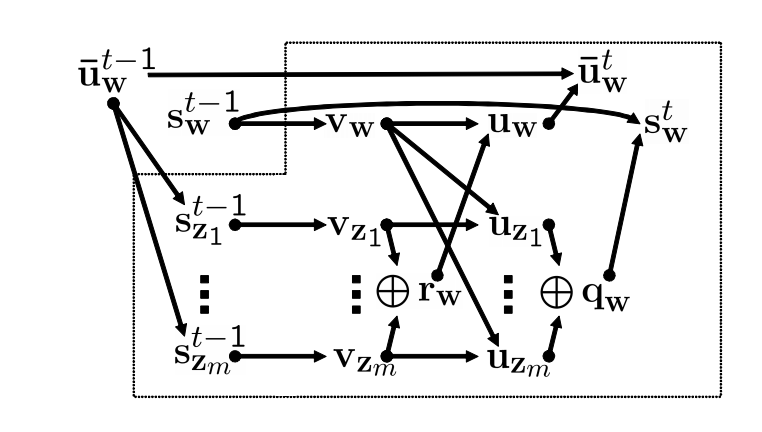
\includegraphics[width=0.8\textwidth]{figures/mem_tweak.png}
  \label{memtweak}
  \caption{Memory efficient algorithm}
\end{figure}

%%% Local Variables:
%%% mode: latex
%%% TeX-master: "mainProject"
%%% End:
